% flashcards-title: Two falling patterns with labeled values
% flashcards-desc: Two small graphs labeled A and B, each with a horizontal axis marked one through four and dots that sit lower as the horizontal value grows. In A three dots on a straight falling line are labeled sixty at one, forty-five at two, and fifteen at four. In B three dots on a curve that falls steeply and then flattens are labeled sixty at one, thirty at two, and fifteen at four.
\documentclass[dvisvgm,tikz,border=8pt]{standalone}
\usepackage{tikz}
\usetikzlibrary{arrows.meta,calc,positioning}
\definecolor{DeckInk}{HTML}{172A3A}
\definecolor{DeckAccent}{HTML}{176B87}
\definecolor{DeckWarm}{HTML}{D97706}
\definecolor{DeckMuted}{HTML}{667784}
\definecolor{DeckPaper}{HTML}{F7FAFC}
\tikzset{
  every node/.style={font=\sffamily, text=DeckInk},
  object/.style={draw=DeckInk, line width=1.1pt, fill=DeckPaper},
  primary/.style={draw=DeckAccent, line width=1.5pt},
  boundary/.style={draw=DeckAccent, line width=1.5pt, dashed, rounded corners=6pt},
  guide/.style={draw=DeckMuted, line width=0.9pt, dashed},
  dimension/.style={{Stealth[length=3.2mm,width=2.2mm]}-{Stealth[length=3.2mm,width=2.2mm]}, draw=DeckWarm, line width=1.2pt},
  motion/.style={-{Stealth[length=3.5mm,width=2.5mm]}, draw=DeckAccent, line width=1.5pt, dashed},
}

\begin{document}
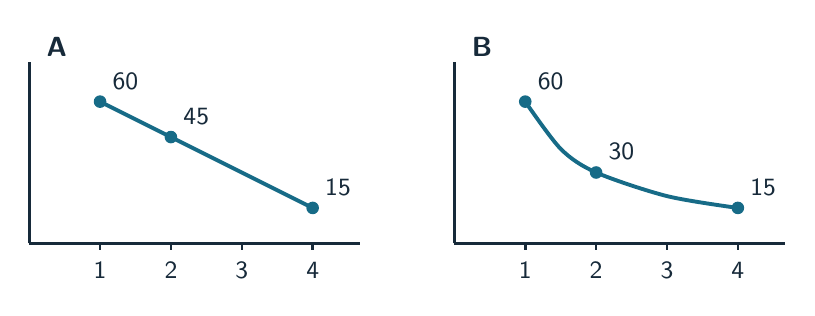
\begin{tikzpicture}[x=1cm,y=1cm]
  % Panel A: straight fall, equal drops (values 60, 45, 15 at 1, 2, 4)
  \draw[DeckInk, line width=1.1pt] (0,0) -- (4.2,0);
  \draw[DeckInk, line width=1.1pt] (0,0) -- (0,2.3);
  \node[font=\sffamily\bfseries] at (0.35,2.5) {A};
  \foreach \x in {1,2,3,4} {
    \draw[DeckInk, line width=0.9pt] (0.9*\x,0) -- (0.9*\x,-0.08);
    \node[font=\sffamily\small, below=1pt of {(0.9*\x,-0.08)}] {\x};
  }
  \draw[DeckAccent, line width=1.4pt] (0.9,1.8) -- (3.6,0.45);
  \fill[DeckAccent] (0.9,1.8) circle (0.08);
  \fill[DeckAccent] (1.8,1.35) circle (0.08);
  \fill[DeckAccent] (3.6,0.45) circle (0.08);
  \node[font=\sffamily\small, above right=1pt and 1pt of {(0.9,1.8)}] {60};
  \node[font=\sffamily\small, above right=1pt and 1pt of {(1.8,1.35)}] {45};
  \node[font=\sffamily\small, above right=1pt and 1pt of {(3.6,0.45)}] {15};
  % Panel B: falling curve, halving pattern (values 60, 30, 15 at 1, 2, 4)
  \begin{scope}[xshift=5.4cm]
    \draw[DeckInk, line width=1.1pt] (0,0) -- (4.2,0);
    \draw[DeckInk, line width=1.1pt] (0,0) -- (0,2.3);
    \node[font=\sffamily\bfseries] at (0.35,2.5) {B};
    \foreach \x in {1,2,3,4} {
      \draw[DeckInk, line width=0.9pt] (0.9*\x,0) -- (0.9*\x,-0.08);
      \node[font=\sffamily\small, below=1pt of {(0.9*\x,-0.08)}] {\x};
    }
    \draw[DeckAccent, line width=1.4pt] plot[smooth]
      coordinates {(0.9,1.8) (1.35,1.2) (1.8,0.9) (2.7,0.6) (3.6,0.45)};
    \fill[DeckAccent] (0.9,1.8) circle (0.08);
    \fill[DeckAccent] (1.8,0.9) circle (0.08);
    \fill[DeckAccent] (3.6,0.45) circle (0.08);
    \node[font=\sffamily\small, above right=1pt and 1pt of {(0.9,1.8)}] {60};
    \node[font=\sffamily\small, above right=1pt and 1pt of {(1.8,0.9)}] {30};
    \node[font=\sffamily\small, above right=1pt and 1pt of {(3.6,0.45)}] {15};
  \end{scope}
\end{tikzpicture}
\end{document}
